\chapter{Électromagnétisme en régime variable}
\label{chap:maxwell}
\section*{Objectifs}
\label{sec:maxwell_objectifs}

\begin{itemize}
	\item Comprendre pourquoi il est nécessaire de modifier les équations 
	  de Maxwell lorsqu'on s'intéresse à un système dépendant du temps
	\item Connaître les équations de Maxwell dans un régime dépendant du temps 
	\item Savoir extraire un contenu physique des équations de Maxwell
	\item Connaître les formes locale et intégrale du bilan d'énergie
	  électromagnétique
	\item Retrouver l'équation de propagation d'une onde électromagnétique
	  dans le vide en utilisant les équations de Maxwell
	\item Connaître la structure spatiale et les propriétés d'une
	  onde électromagnétique progressive plane
	\item Comprendre comment est modifiée la propagation d'une onde 
	  électromagnétique par la présence d'un conducteur
\end{itemize}

\section*{Introduction}

\section{Les limites des équations en régime permanent}
Malheureusement la forme des équations de Maxwell en régime permanent n'est pas
totalement compatible avec les comportements électromagnétiques observés en régime 
variable. En effet, ces lois présentent des incohérences internes et ne permet
pas de décrire tous les résultats expérimentaux.

\subsection{Équation de conservation de la charge}
Dans cette section, on s'intéresse à l'équation de conservation de la charge
que nous allons démontrer dans le cas 1D et généraliser au cas 3D. Nous allons
pour ce faire sortir temporairement du régime permanent et considérer des
grandeurs dépendantes du temps.

On se place dans un repère cartésien $(O, \ex)$. La position d'un point 
de l'espace $P$ est donc repérée par sa coordonnée $x$. On considère un volume
infinitésimale de section $S$ compris entre les abscisses $x$ et $x + \dx$.
Ce volume possède une densité volumique de charge $\rho(x, t)$. Les charges se 
déplacent selon un mouvement d'ensemble caractérisé par un vecteur densité de 
courant électrique $\vecj(x, t) = j(x, t)\ex$ 
(voir Fig.~\ref{fig:conservation_charge}). 

\begin{figure}[htpb]
	\centering
	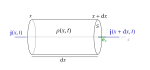
\includegraphics[scale=0.9]{conservation_charge}
	\caption{Volume élémentaire $S\dx$ sur lequel on effectue le bilan
	de charges électriques.}
	\label{fig:conservation_charge}
\end{figure}
On cherche à déterminer une équation qui relie $\rho$ à $\vecj$. Pour ce faire
on exprime la différence entre la charge $Q(t + \dt)$ contenue dans le volume
à l'instant $t + \dt$ et la charge $Q(t)$ contenue à l'instant $t$ de deux manières
différentes.

\begin{enumerate}
	\item $Q(t)$ s'obtient en multipliant la densité volumique de charge $\rho(x, t)$
	par le volume $S \dx$. On a alors 
	\begin{equation*}
		Q(t + \dt) - Q(t) = [\rho(x, t + \dt) - \rho(x, t)] S\dx.
	\end{equation*}

	\item D'autre part, le mouvement d'ensemble des charges entraîne un 
	  flux entrant $j(x, t) \cdot S \dt$ et un flux sortant 
	  $j(x + \dx, t) \cdot S \dt$ de charges à travers la
	  surface délimitant $V$. On a alors
	  \begin{equation*}
		  Q(t + \dt) - Q(t) = [j(x, t) - j(x + \dx, t)]S \dt.
	  \end{equation*}
\end{enumerate}
Ces deux équations nous permettent d'aboutir à l'équation de conservation de la
charge en 1D
\begin{equation*}
	[\rho(x, t + \dt) - \rho(x, t)] S \dx = -[j(x + \dx, t) - j(x, t)] S \dt
	\iff \boxed{\dd{\rho}{t}(x, t) = - \dd{j}{x}.}
\end{equation*}

\begin{defn}[Équation de conservation de la charge]
	En tout point $M$ de l'espace, la densité volumique de charge $\rho$
	et le vecteur densité de courant $\vecj$ 
	vérifie l'équation de conservation de la charge
	\begin{equation*}
		\dd{\rho}{t}(M, t) + \div \vecj(M, t) = 0.
	\end{equation*}
\end{defn}

Le vecteur densité de courant $\vecj$ apparaît à la fois dans l'équation 
de conservation de la charge et dans l'équation de Maxwell-Ampère. Ces deux
équations sont-elles compatibles ?

Soit un champ magnétique $\vecb$ et un vecteur densité de courant $\vecj$ 
associé. L'équation locale de Maxwell-Ampère s'écrit en tout pont de l'espace
\begin{equation*}
	\rot \vecb = \mu_0 \vecj.
\end{equation*}
On peut alors déterminer l'expression de $\div \vecj$
\begin{equation*}
	\div \vecj = \dfrac{1}{\mu_0} \div(\rot \vecb) = 0
\end{equation*}
car $\div(\rot \vecb) = 0$. Or cette égalité n'est vérifiée qu'en régime permanent 
$\left(\dd{\rho}{t} = 0 \right)$!

Maxwell proposa en 1864 d'ajouter à l'équation~\ref{eq:magneto_ma} un nouveau terme 
$\vecj_D$ qu'il nomme \textbf{courant de déplacement}
\begin{equation*}
	\rot \vecb = \mu_0 (\vecj + \vecj_D).
\end{equation*}
Quelle est alors l'expression de $\vecj_D$ ? D'après l'équation de conservation 
de la charge, $\vecj$ vérifie 
\begin{equation*}
	\div \vecj = -\dd{\rho}{t},
\end{equation*}
où $\rho$ est la densité volumique de charge. Or d'après l'équation de Maxwell-Ampère, 
la divergence de $\vecj$ doit aussi vérifier
\begin{equation*}
	\div \vecj = \div \left(\dfrac{\rot \vecb}{\mu_0} - \vecj_D \right)
	        = - \div(\vecj_D),
\end{equation*}
car la divergence d'un rotationnel est nul.
En utilisant l'équation locale de Maxwell-Gauss, on montre alors
que $\vecj_D$ doit vérifier
\begin{equation}
	\div \left(\vecj_D - \epsilon_0 \dd{\vece}{t}\right) = 0 \Rightarrow 
	\boxed{\vecj_D = \epsilon_0 \dd{E}{t}.}
	\label{eq:deplacement}
\end{equation}

\begin{rem}
	$\epsilon_0 \dd{E}{t}$, n'est pas la seule solution à 
	l'équation~\ref{eq:deplacement}. En effet, cette solution est définie
	à un rotationnel près. Maxwell a choisi pour expression de $\vecj_D$
	la solution la plus simple. Ce choix a ensuite été confirmé par des 
	résultats expérimentaux.
\end{rem}

Finalement, l'équation de Maxwell-Ampère s'écrit
\begin{equation}
	\boxed{\rot \vecb = \mu_0 \left( \vecj + \epsilon_0 \dd{\vece}{t} \right).}
\end{equation}
\subsection{Équation de Maxwell-Faraday et phénomènes d'induction}
Les phénomènes d'induction électromagnétique ont été découverts en 1831
par Michael Faraday ($1791-1867$). Il montre alors que des courants induits 
se développent dans un 
circuit immobile plongé dans un champ magnétique variable alors que ce dernier
n'est alimenté par aucun générateur. Ce phénomène n'est pas décrit par
les équations de la magnétostatique et de l'électrostatique.

\section{Les équations de Maxwell}
Nous allons maintenant nous concentrer sur les équations de Maxwell en régime 
variable et sur leur interprétation physique. Pour ce faire nous les
présentons comme deux jeux de deux équations.

\begin{defn}[Équations de Maxwell structurelles]
	Les équations de \textbf{Maxwell-Faraday}
	\begin{equation}
		\rot \vece = - \dd{\vecb}{t} \iff \oint_\mathcal{C} \vece 
		\cdot \dl = - \dd{\phi}{t},
	\end{equation}
	où $\phi$ est le flux du champ magnétique $\vecb$ à travers la 
	surface qui s'appuie sur n'importe quel contour fermé $\mathcal{C}$, 
	et \textbf{Maxwell-Thomson}
	\begin{equation}
		\div \vecb = 0 \iff \oiint_\mathcal{S} \vecb \cdot \ds = 0,
	\end{equation}
	où $\mathcal{S}$ est une surface fermée quelconque, ne relient pas les champs 
	électrique $\vece$ et magnétique $\vecb$
	au vecteur densité de courant $\vecj$ et à la densité volumique de 
	charge $\rho$. Elles sont donc indépendantes du milieu considéré.
\end{defn}

On remarque rapidement que l'équation de Maxwell-Thomson reste inchangée par rapport
à ce que nous avons vu en magnétostatique (voir Chap.~\ref{chap:magnetostatique}).
En revanche, l'équation de Maxwell-Faraday fait maintenant apparaître le
champ magnétique ! Cette relation signifie
qu'un champ magnétique variant dans le temps peut donner naissance à un champ électrique
dont le rotationnel est non nul. Cette relation décrit le phénomène d'induction 
électromagnétique et met en avant une seconde source de champ électrique: 
un champ magnétique variable dans le temps. 

\begin{attention}
	Si $\vece$ est un champ électrique à rotationnel non nul, la relation 
	$\vece = - \grad V$, où $V$ est le potentiel électrique, n'est plus valide.
\end{attention}

\begin{defn}[Équations de Maxwell couplées à la matière]
	En revanche les équations de \textbf{Maxwell-Gauss}
	\begin{equation}
		\div \vece = \dfrac{\rho}{\epsilon_0} \iff \oiint_\mathcal{S}
		\vece \cdot \ds = \dfrac{Q}{\epsilon_0}, 
	\end{equation}
	où $Q$ est la charge contenue dans la surface fermée $\mathcal{S}$ quelconque, 
	et de \textbf{Maxwell-Ampère} 
	\begin{equation}
		\rot \vecb = \mu_0\left(\vecj + \epsilon_0 \dd{\vece}{t}\right)
		\iff \oint_\mathcal{C} \vecb \cdot \dl = \mu_0 \left[
		I + \epsilon_0 \dfrac{\partial}{\partial t} 
		\left(\iint \vece \cdot \ds\right)
	\right],
	\end{equation}
	où $I$ est le courant enlacé par le contour fermé $\mathcal{C}$ quelconque, 
	lient les champs électrique $\vece$ et magnétique $\vecb$ à leur source 
	modéliser par le vecteur densité
	de courant $\vecj$ et la densité volumique de charge $\rho$. 
\end{defn}

L'équation de Maxwell-Gauss reste de même inchangée par le passage en régime
dépendant du temps. En revanche, l'équation de Maxwell-Ampère fait apparaître un
second terme, $\vecj_D = \epsilon_0 \dd{\vece}{t}$, appelé \textbf{courant de
déplacements}. Un champ électrique variant dans le temps devient alors, au même
titre qu'un courant, une source de champ magnétique. Ce second terme à un rôle
analogue au terme $- \dd{\vecb}{t}$ apparaissant dans l'équation de 
Maxwell-Faraday, il induit un couplage du champ électrique et du champ magnétique
qui ne peuvent plus être dissociés comme c'était le cas en magnétostatique
et en électrostatique.

\begin{attention}
	La dénomination courant de déplacement,
	donnée par Maxwell lui-même, 
	pour le second terme de l'équation de Maxwell-Ampère est trompeuse
	car ce terme n'est associé ni à un déplacement, ni à à un courant !
\end{attention}

Il est important de remarquer que les équations de Maxwell sont linéaires.
Le principe de superposition est donc toujours vérifié en régime variable. 

\begin{exemple}
	Si les champs électromagnétiques $(\vece_1, \vecb_1)$ et 
	$(\vece_2, \vecb_2)$ vérifient les équations de Maxwell, alors le champ
	électromagnétique $(\vece_1 + \vece_2, \vecb_1 + \vecb_2)$ les vérifie
	aussi.
\end{exemple}

\section{Énergie électromagnétique}
Comme un système matériel, le champ électromagnétique est caractérisé par une énergie.
On constate d'ailleurs en électrocinétique que les condensateurs et les bobines sont
capables de stocker de l'énergie électrique et magnétique. Le but de cette partie
est donc de déterminer l'expression de cette énergie en faisant apparaître le
champ électrique $\vece$ et le champ magnétique $\vecb$.

On propose de réaliser un bilan d'énergie sur un volume
$V$ de l'espace délimité par une surface $\mathcal{S}$ 
immobile dans le référentiel d'étude supposé galiléen 
(voir Fig.~\ref{fig:bilan_energie}). 

\begin{figure}[htpb]
	\centering
	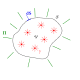
\includegraphics[scale=0.9]{bilan_energie}
	\caption{Volume sur lequel on réalise le bilan d'énergie.
	Ce volume contient des sources internes (en rouge) de densité volumique
	de puissance $\gamma$. L'énergie qui traverse la surface $\mathcal{S}$
	(en vert) est caractérisée par une densité surfacique de flux par unité 
	de temps $\mathbf{\Pi}$.}
	\label{fig:bilan_energie}
\end{figure}
Comme
cela a été fait pour la conservation de la charge, nous cherchons alors à
déterminer comment varie l'énergie $\mathcal{E}$
contenue dans ce volume au cours du temps entre un instant $t$ et un instant
$t + \dt$. Cette variation 
$\mathcal{E}(t + \dt) - \mathcal{E}(t)$ 
d'énergie peut résulter

\begin{enumerate}
	\item de la présence de sources d'énergie à l'intérieur
	  du volume. Elles lui fournissent durant une durée $\dt$ une énergie
	  $\delta \mathcal{E}_\mathrm{source}$
	  \begin{equation*}
		  \delta \mathcal{E}_\mathrm{source} = 
		  \iiint_{P \in V} \gamma(P, t) \dV \dt,
	  \end{equation*}
	  où $\gamma$ $(\joule \usk \rpcubic \meter \usk \rp \second)$ 
	  correspond à la densité volumique de puissance 
	  reçue par le volume de la part de ces sources, 
	  c'est-à-dire la quantité d'énergie reçue par unité de temps et de 
	  volume.
  	\item d'un flux d'énergie à travers la surface $\mathcal{S}$ qui délimite le volume
    	$V$. On note ici $\ds$ le vecteur surface élémentaire dirigé vers l'extérieur
	du volume. On définit alors une densité surfacique de flux d'énergie 
	par unité de temps $\mathbf{\Pi}$ ($\joule \usk \meter \rpsquared
	\usk \rp \second$). L'énergie traversant la surface $\mathcal{S}$ par unité de 
	temps s'écrit alors
	\begin{equation*}
		\delta \mathcal{E}_\mathrm{flux} = - \oiint_{P \in \mathcal{S}}
		\mathbf{\Pi}(P, t) \cdot \ds \dt.
	\end{equation*}
	Lorsque cette quantité est positive, l'énergie est reçue par le volume.
	En revanche, lorsqu'elle est négative, l'énergie est transmise à l'extérieur
	par le volume.
\end{enumerate}
Finalement, on aboutit à
\begin{equation*}
	\boxed{\dn{\mathcal{E}}{t}(t) = \iiint_{P \in \mathcal{V}} \gamma(P, t) \dV
	- \oiint_{P \in mathcal{S}} \mathbf{\Pi}(P, t) \cdot \ds.}
\end{equation*}

\begin{defn}[Bilan d'énergie]
	Soit un volume $V$ de l'espace immobile 
	dans le référentiel d'étude supposé
	galiléen et délimité par une surface $\mathcal{S}$. La variation 
	temporelle de l'énergie $\mathcal{E}(M, t)$
	contenue dans le volume est liée à
	\begin{enumerate}
	\item la densité volumique de puissance
	$\gamma$, mesurée en $\watt \usk \rpcubic \meter$ 
	  $(\joule \usk \rpcubic \meter \usk \rp \second)$, 
	  reçue algébriquement par le système de la part de sources internes,
	
  	\item la densité surfacique de flux d'énergie $\vec{\Pi}$,
	  mesurée en $\watt \usk \meter \rpsquared$ 
	  $(\joule \usk \meter \rpsquared \usk \rp \second)$,
	  traversant la surface $\mathcal{S}$,
	\end{enumerate}
	
	\begin{equation}
		\dn{\mathcal{E}}{t}(t) = \iiint_{P \in \mathcal{V}} \gamma(P, t) \dV
		- \oiint_{P \in \mathcal{S}} \vec{\Pi}(P, t) \cdot \ds.
	\end{equation}

	Ce bilan d'énergie est décrit localement en un point $M$ de l'espace
	par l'équation
	\begin{equation}
		\dd{w}{t}(M, t) = -\div \vec{\Pi}(M, t) + \gamma(M, t),
	\end{equation}
	où $w$ est la densité volumique d'énergie 
	mesurée en $\joule \usk \rpcubic \meter$.
\end{defn}

Le but est maintenant d'obtenir une formule similaire pour le champ électromagnétique
$(\vece, \vecb)$ afin de déterminer les expressions de
$w$, $\mathbf{\Pi}$ et $\gamma$ dans ce cas. L'équation de Maxwell-Ampère 
permet d'obtenir

\begin{equation*}
	\rot \vecb = \mu_0\left(\vecj + \epsilon_0 \dd{\vece}{t} \right)
	\iff 
	\rot \vecb \cdot \vece = \mu_0\left(\vecj \cdot \vece + 
	\epsilon_0 \dd{\vece}{t} \cdot \vece \right),
\end{equation*}
où $\vecj$ est le vecteur densité de courant.
On peut alors se servir de l'identité vectorielle $\div(\vec{W} \wedge
\vec{Y}) = \vec{Y} \cdot \rot \vec{W} - \vec{W} \cdot \rot \vec{Y}$, vérifiée
pour tous vecteurs $\vec{W}$ et $\vec{U}$, pour transformer le terme de 
gauche de l'équation précédente
\begin{equation*}
	- \div (\vece \wedge \vecb) + \vecb \cdot \rot \vece =
	\mu_0\left(\vecj \cdot \vece + \epsilon_0 \dd{\vece}{t} \cdot \vece \right).
\end{equation*}
On peut alors remplacer $\rot \vece$ en utilisant l'équation de Maxwell-Faraday
\begin{equation*}
	- \div (\vece \wedge \vecb) - \vecb \cdot \dd{\vecb}{t} =
	\mu_0\left(\vecj \cdot \vece + \epsilon_0 \dd{\vece}{t} \cdot \vece \right)
	\Rightarrow
	\boxed{\dfrac{\partial}{\partial t} \left(\dfrac{\epsilon_0 \vece^2}{2}
		+ \dfrac{\vecb^2}{2 \mu_0} \right) = - \div\left(
\dfrac{\vece \wedge \vecb}{\mu_0}\right) - \vecj \cdot \vece.}
\end{equation*}

\begin{defn}[Bilan d'énergie électromagnétique]
	Soit un volume $V$ de l'espace immobile dans le référentiel d'étude supposé
	galiléen et délimité par une surface $\mathcal{S}$. La variation 
	temporelle de l'énergie $\mathcal{E}_\mathrm{em}(t)$ électromagnétique
	contenue dans le volume est liée à
	\begin{enumerate}
	\item la densité volumique de puissance électromagnétique
		$- \vecj \cdot \vece$ ($\watt \usk \rpcubic \meter$) 
	  reçue algébriquement par le système de la part de sources internes,
	
	\item la densité surfacique de flux d'énergie électromagnétique $\mathbf{\Pi}$
		($\watt \usk \meter \rpsquared$),
  	  appelé \textbf{vecteur de Poynting}, traversant la surface $\mathcal{S}$
	\end{enumerate}
	
	\begin{equation}
		\dn{\mathcal{E}}{t}(t) = - \iiint_{P \in \mathcal{V}} 
		\vecj(P, t) \cdot \vece(P, t) \dV 
		- \oiint_{P \in \mathcal{S}} \mathbf{\Pi}(P, t) \cdot \ds,
	\end{equation}
	avec
	\begin{equation}
		\mathbf{\Pi}(P, t) = \dfrac{\vece(P, t) \wedge \vecb(P, t)}{\mu_0}.
	\end{equation}

	Ce bilan d'énergie est décrit localement en un point $M$
	par l'équation
	\begin{equation}
		\dd{w}{t}(M, t) = -\div \mathbf{\Pi}(M, t) + \gamma(M, t),
	\end{equation}
	où $w_\mathrm{em}$ $(\joule \usk \meter \rpcubic)$ 
	est la densité volumique d'énergie électromagnétique définie par
	\begin{equation}
		w_\mathrm{em}(M, t) = \dfrac{\epsilon_0 \vece^2(M, t)}{2} 
		+ \dfrac{\vecb^2(M, t)}{2 \mu_0}.
	\end{equation}
\end{defn}

\section{Ondes électromagnétiques dans le vide}
Les équations de Maxwell, en plus de fournir un cadre mathématique solide 
à l'électromagnétisme, prévoient l'existence des ondes électromagnétiques. 
En effet, le couplage des champs électrique $\vece$ et magnétique $\vecb$ 
rend possible la propagation d'une perturbation du champ électromagnétique
$(\vece, \vecb)$. 

\cite{Gie1985b} proposent une approche intuitive du phénomène
qui permet de mieux le comprendre. Imaginons la naissance d'une perturbation 
du champ électrique $\vece$ localisée en une région de l'espace. Cette perturbation
donne naissance à un champ magnétique $\vecb$ dans son voisinage par l'intermédiaire des 
courants de déplacements. Ce même champ magnétique, par l'intermédiaire de 
l'équation de Maxwell-Faraday, génère un champ électrique. La perturbation se 
propage de proche en proche.

\subsection{Équation de propagation du champ magnétique}
Soient un champ magnétique $\vecb$ et un champ électrique $\vece$ dans une région
vide de l'espace, c'est-à-dire avec une densité volumique de charge $\rho$ 
et un vecteur densité de courant $\vecj$ nuls en tout point de l'espace. 
Les évolution spatiale et temporelle de ces deux champs sont contrôlées par les équations
de Maxwell dans le vide

\begin{equation*}
\div \vece = 0,\quad \rot \vecb = \mu_0 \epsilon_0 \dd{\vece}{t},\quad
\rot \vece = -\dd{\vecb}{t} \quad \mathrm{et} \quad \div \vecb = 0.
\end{equation*}

Nous allons essayer en combinant ces équations d'obtenir une équation combinant
les variations temporelles et spatiales du champ magnétique. Pour cela, on 
commence par faire apparaître $\rot \vece$ dans l'équation de Maxwell-Ampère

\begin{equation*}
	\rot(\rot \vecb) = \mu_0 \epsilon_0 \rot \dd{\vece}{t}.
\end{equation*}
Il est alors possible de permuter le rotationnel et la dérivée temporelle, puis
de remplacer $\rot \vece$ par son expression en se servant de l'équation de 
Maxwell-Faraday

\begin{equation*}
	\rot(\rot \vecb) = -\mu_0 \epsilon_0 \dd{^2\vecb}{t^2}.
\end{equation*}
Finalement, en utilisant la relation $\rot(\rot \vecb) = - \laplacien \vecb 
+ \gradient(\div \vecb)$ et l'équation de Maxwell-Thomson, on obtient
\begin{equation*}
	\boxed{\laplacien \vecb - \mu_0 \epsilon_0 \dd{^2\vecb}{t^2} = \mathbf{0}}.
\end{equation*}
Cette équation, dite de \textbf{d'Alembert}, couple les variations temporelles
et spatiales du champ magnétique $\vecb$. Elle est caractéristique du phénomène
de propagation d'onde. De la même manière, le champ électrique vérifie
\begin{equation*}
	\boxed{\laplacien \vece - \mu_0 \epsilon_0 \dd{^2\vece}{t^2} = \mathbf{0}}.
\end{equation*}
On constate la présence du facteur $\mu_0 \epsilon_0$ dans cette équation. 
À quoi ce terme correspond-il ? On remarque que d'après l'équation précédente, ce 
facteur doit être homogène à l'inverse du carré d'une vitesse. 
On se propose de vérifier cela avec les dimensions de $\epsilon_0$ 
et $\mu_0$. La permittivité diélectrique du vide $\epsilon_0$ s'exprime en 
$\rp \kilogram \usk \rpcubic \meter \usk \second^4 \usk \ampere \squared$ 
tandis que la perméabilité magnétique du vide $\mu_0$ s'exprime en 
$\kilogram \usk \meter \usk \rpsquare \second \usk \rpsquare \ampere$, 
$\epsilon_0 \mu_0$ est donc homogène à l'inverse du carré d'une vitesse. Ce facteur
correspond donc à la vitesse de propagation $c$ d'une onde électromagnétique. 
Cette vitesse vaut
\begin{equation*}
	c = \dfrac{1}{\sqrt{\epsilon_0 \mu_0}} = \unit{299\ 792\ 458}{\meter 
	\usk \rp \second},
\end{equation*}
correspondant ainsi à la vitesse de la lumière dans le vide.

\begin{rem}
	Contrairement aux ondes mécaniques, les ondes électromagnétiques ne
	nécessitent pas de milieux pour se propager. Elles y arrivent très bien
	dans le vide.
\end{rem}

\begin{defn}[Équation de propagation du champ électromagnétique]
	Les propagations des champs électrique $\vece$ et magnétique $\vecb$ obéissent 
	à la même équation de d'Alembert en un point $M$ de l'espace
	\begin{equation}
	\laplacien \vece(M, t) - \mu_0 \epsilon_0 \dd{^2\vece}{t^2}(M, t) = \mathbf{0}
	\quad \mathrm{et} \quad
	\laplacien \vecb(M, t) - \mu_0 \epsilon_0 \dd{^2\vecb}{t^2}(M, t) = \mathbf{0},
	\end{equation}
	leur célérité étant donnée par 
	\begin{equation*}
		c = \dfrac{1}{\sqrt{\epsilon_0 \mu_0}}.
	\end{equation*}
	$c$ correspond ici à la vitesse de la lumière dans le vide. Cette équation
	de propagation a le bon goût d'être linéaire. De plus, si on change $t$
	en $-t$ l'équation demeure la même.
\end{defn}

\begin{rem}
	L'équation de de d'Alembert est une équation caractéristique des phénomènes
	de propagation sans dissipation.
\end{rem}

Les champ électrique $\vece$ et magnétique $\vecb$ sont des champs vectoriels.
Chacune de leurs composantes vérifie l'équation de d'Alembert.

\subsection{Solutions de l'équation de d'Alembert}
Nous considérons maintenant le cas de l'équation de d'Alembert à une dimension.
On se place dans un repère cartésien $(O, \ex, \ey, \ez)$ et on considère
un champ électrique de la forme $\vece(x, t) = E(x, t)\ey$.
La propagation du champ électrique $\vece$ dans ce repère vérifie alors 
\begin{equation*}
	\dd{^2 E}{x^2}(x, t) - \mu_0 \epsilon_0 \dd{^2 E}{t^2}(x, t) = \mathbf{0}.
\end{equation*}
La solution générale de cette équation s'écrit sous la forme
\begin{equation*}
	E(x, t) = E_+\left(t - \frac{x}{c}\right) + E_- \left(t + \frac{x}{c}\right),
\end{equation*}
où $E_+$ correspond à une ondes électromagnétiques qui se déplacent vers 
les $x$ décroissants, tandis que $E_-$ correspond à une onde se déplaçant vers 
les $x$ croissants.

\begin{rem}
	Le phénomène de propagation correspond à un couplage du temps et 
	de l'espace par la vitesse de propagation. En effet, on remarque que 
	la solution générale de l'équation de d'Alembert réunit les variables
	temporelle et spatiale en une seule variable.
\end{rem}

Pour mieux comprendre ce phénomène de propagation, il peut être utile de prendre
le cas d'une onde mécanique. Imaginons alors une corde dont on viendrait secouer par un
geste brusque et rapide une des extrémités. Ce mouvement donne alors naissance
à la propagation d'une onde le long de la corde


On se place dans un repère cartésien $(O, \ex, \ey)$. 
 Au repos, un point $M$ de la corde occupe la coordonnée $(x, 0)$.
À l'instant $t = 0$, la corde est excitée à son extrémité en 
$x = 0$. La perturbation induite par le passage de l'onde modifie la position
du point $M$ qui devient $(x, y)$ (voir Fig.~\ref{fig:maxwell_corde}), 
où la variable $y$ vérifie l'équation de 
d'Alembert. L'onde se propageant vers les $x$ croissants, $y$ est de la forme

\begin{equation*}
	y(x, t) = y\left(t - \frac{x}{v}\right),
\end{equation*}
où $v$ est la vitesse propagation de l'onde. On peut alors déterminer $y$ pour
$x = x + \Delta x$ avec $\Delta x = v \Delta t$ à l'instant $t + \Delta t$

\begin{equation*}
	y\left(x + v \Delta t, t + \Delta t\right) = y\left(t + \Delta t - 
	\frac{x + v \Delta t}{v}\right) = y\left(t - \dfrac{x}{v}\right).
\end{equation*}
On remarque alors que l'ordonnée du point d'abscisse $x + v \Delta t$ à l'instant
$t + \Delta t$ correspond exactement à l'ordonnée du point d'abscisse $x$
à l'instant $t$ (voir Fig.~\ref{fig:maxwell_corde}). La perturbation s'est propagée
sans déformation.

\begin{rem}
	Cette non-déformation de la propagation illustre la réversibilité temporelle
	de l'équation de d'Alembert.
\end{rem}

\begin{figure}[htpb]
	\centering
	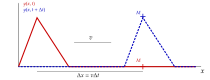
\includegraphics[width=0.7\linewidth]{corde}
	\caption{Propagation d'une onde mécanique entre les dates $t$ (en rouge) et $t
	+ \Delta t$ (en bleu tirets). Cette onde se propage à la vitesse $v$. Elle
	entraîne une déformation transverse de la corde.}%
	\label{fig:maxwell_corde}
\end{figure}

\subsection{Ondes planes progressives harmoniques}
\subsubsection{Champ électromagnétique et ondes planes progressives harmoniques}
Nous allons dans ce cours nous focaliser sur une famille particulière de solutions
à l'équation de d'Alembert: les \textbf{ondes planes progressives harmoniques}
(OPPH). En effet, les OPPH forment une base de l'espace des solutions de l'équation
de d'Alembert. Toute fonction solution de cette équation peut se décomposer en une
superposition d'OPPH. Cette décomposition est rendue possible
par la linéarité de l'équation de d'Alembert.

Une OPPH est caractérisée par 
\begin{itemize}
	\item sa fréquence $f$ (en $\hertz$) ou sa pulsation temporelle $\omega$ 
		(en $\rad \usk \rp \second$) ou sa période temporelle $T$ (en $\second$)
	  avec
	  \begin{equation*}
		  T = \frac{1}{f} = \frac{2\pi}{\omega}.
	  \end{equation*}
  	\item sa pulsation spatiale $k$ (en $\rad \usk \rp \meter$) ou 
	  sa longueur d'onde $\lambda$ (en $\meter$) avec 
	  \begin{equation*}
		  \lambda = \dfrac{2 \pi}{k}.
	  \end{equation*}
	\item sa direction de propagation $\vec{u}$.
\end{itemize}

Chaque composante $E_i$ et $B_i$ des champs électrique et magnétique en un point 
$M$ de l'espace s'écrit alors
sous la forme
\begin{equation*}
	E_i(M, t) = E_{i, 0}\cos(\omega t - \vec{k} \cdot \vec{r} + \phi_i)
	\quad \mathrm{et} \quad
	B_i(M, t) = B_{i, 0}\cos(\omega t - \vec{k} \cdot \vec{r} + \psi_i),
\end{equation*}
où $\vec{k} = k \vec{u}$ est le vecteur d'onde, $E_{i, 0}$ et $B_{i, 0}$ 
sont les amplitudes des champs, 
$\vec{r} = \vec{OM}$ est le vecteur position du point considéré
et $\phi_i$ et $\psi_i$ les phases à l'origine. 
Dans ce cours, nous utiliserons par commodité la notation complexe
\begin{equation*}
	\boxed{
		\complex{E_i}(M, t) = \complex{E_{i, 0}}\exp[i(
		\omega t - \vec{k} \cdot \vec{r})]
	\quad \mathrm{et} \quad
\complex{B_i}(M, t) = \complex{B_{i, 0}}\exp[i(\omega t - \vec{k} \cdot \vec{r})]},
\end{equation*}
avec $\complex{B_{i, 0}} = B_{i, 0} \exp(\psi_i)$ et 
$\complex{E_{i, 0}} = E_{i, 0} \exp(\phi_i)$. On retrouve alors les champs réels
en prenant la partie réelle des champs complexes.

\begin{rem}
Les longueurs d'ondes et fréquences des ondes électromagnétiques couvrent un large
domaine comme le soulignent la figure~\ref{fig:maxwell_spectre}.
\end{rem}

\begin{figure}[]
	\centering
	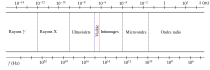
\includegraphics[scale=0.7]{spectre}
	\caption{Ensemble du spectre des ondes électromagnétiques en précisant
	la longueur d'onde $\lambda$ et la fréquence $f$ de chaque domaine. Le
	domaine du visible se situe entre $\unit{400}{\nano \meter}$ et
	$\unit{800}{\nano \meter}$.}%
	\label{fig:maxwell_spectre}
\end{figure}

\subsubsection{Relation de dispersion}
On peut alors se demander à quelle condition une OPPH est solution de l'équation de
d'Alembert.
Pour ce faire, on remplace les composantes des champs électrique et magnétiques 
par leur expression dans l'équation de d'Alembert. Pour une composante 
$\complex{E_i}$ du champ électrique en un point $M$ de l'espace cela donne
\begin{equation*}
	\Delta \complex{E_i}(M, t) -\dfrac{1}{c^2} \dd{^2\complex{E_i}}{t^2}(M, t) = 0
	\iff (-ik)^2 \complex{E_i}(M, t) - \dfrac{\omega^2}{c^2} 
	\complex{E_i}(M, t) = 0.
\end{equation*}
Comme cette relation est vérifiée en tout point de l'espace on aboutit à la relation
\begin{equation*}
	\boxed{
	k = \frac{\omega}{c}.
	      }
\end{equation*}

\begin{defn}[Relation de dispersion de l'équation de d'Alembert]
	Soit une OPPH de pulsation temporelle $\omega$, de pulsation 
	spatiale $k$ se déplaçant à une vitesse $c$. Cette OPPH est solution
	de l'équation de d'Alembert si ces trois grandeurs vérifient la
	relation de dispersion
	\begin{equation}
		k = \dfrac{\omega}{c}.
	\end{equation}
	La période temporelle $T$ de l'onde est alors reliée à sa longueur d'onde
	$\lambda$ par la relation 
	\begin{equation}
		\lambda = c T.
	\end{equation}
	En d'autres termes, la longueur d'onde est la distance parcourue par l'onde
	en une période. En résumé, la relation de dispersion relie les 
	dimensions spatiales et temporelles de l'onde.
\end{defn}

\subsubsection{Équations de Maxwell et ondes planes progressives harmoniques}
Il devient alors possible d'écrire les équations de Maxwell sous une forme
dite complexe. Il est pour cela nécessaire de savoir ce que deviennent 
les opérateurs divergence et rotationnel en notation complexe. 

On se place dans un repère cartésien $(O, \ex, \ey, \ez)$.
Soit $\vec{A}$ un champ vectoriel dont les variations temporelles et spatiales de 
chacune de ses composante sont décrites par une OPPH de pulsation temporelle 
$\omega$ et de vecteur d'onde $\vec{k}$. En un point $M (x, y, z)$ de l'espace, 
chaque composante de
$\vec{A}$ s'écrit sous forme complexe
\begin{equation*}
	\complex{A_i}(M, t) = \complex{A_{i, 0}}\exp[i(\omega t - \vec{k} 
	\cdot \vec{OM})],
\end{equation*}
avec $\vec{k} = k_x\ex + k_y\ey + k_z\ez$, $\vec{OM} = x\ex + y\ey +z\ez$
et $\complex{A_{i, 0}}$ l'amplitude complexe de $\complex{A}$.
On peut alors exprimer la divergence de ce champ vectoriel dans le référentiel choisi
\begin{equation*}
	\div \complex{A}(M, t) = \dd{\complex{A}_x}{x}(M, t) + 
	\dd{\complex{A}_y}{y}(M, t) + \dd{\complex{A}_z}{z}(M, t).
\end{equation*}
Si on s'intéresse à la premier composante, cela donne
\begin{equation*}
	\dd{\complex{A}_x}{x}(M, t) = \complex{A_{x, 0}} \dd{}{x}
	\exp[i(wt - k_x x - k_y y -k_z z)] =
	-i k_x \complex{A_{x, 0}} 
	\exp[i(wt - k_x x - k_y y -k_z z)] = -i k_x \complex{A}_x(M, t).
\end{equation*}
Finalement, la divergence de $\complex{A}$ s'exprime en notation complexe
\begin{equation*}
	\boxed{
	\div \complex{\vec{A}}(M, t) = -i \vec{k} \cdot \complex{\vec{A}}(M,t)
}
\end{equation*}
De la même manière, on peut montrer que 
\begin{equation*}
	\boxed{
	\rot \complex{\vec{A}}(M, t) = -i \vec{k} \wedge \complex{\vec{A}}(M, t).
	}
\end{equation*}

\begin{figure}[b]
	\centering
	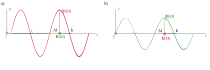
\includegraphics[scale=0.9]{structure}
	\caption{Structure spatiale d'une onde électromagnétique plane progressive
	harmonique de fréquence $f$, de longueur d'onde $\lambda$ et de vecteur d'onde 
$\vec{k}$ dans le plan $(O, \ex, \ey)$ à gauche et dans le plan $(O, \ex, \ez)$
à droite.}%
	\label{fig:maxwell_structure}
\end{figure}

\begin{defn}[Équations de Maxwell en notation complexe]
Soit un champ électrique $\vece$ et un champ magnétique $\vecb$
dont les variations spatiales et temporelles de chaque composante sont décrites 
par une OPPH de vecteur d'onde $\vec{k}$ et de pulsation $\omega$. Ces deux champs 
vectoriels vérifient les équations de Maxwell qui s'écrivent en notation complexe

\begin{description}[labelindent=2em, itemsep=1em]
	\item[Maxwell-Gauss: ]
		$\vec{k} \cdot \complex{\vece}(M, t) = 0$,
	\item[Maxwell-Thomson: ] $\vec{k} \cdot \complex{\vecb}(M, t) = 0$,
	\item[Maxwell-Faraday: ]
		$\vec{k} \wedge \complex{\vece}(M, t) = \omega \complex{\vecb}(M, t)$,
	\item[Maxwell-Ampère: ]
		$\vec{k} \wedge \complex{\vecb}(M, t) = - \dfrac{\omega}{c^2}
		\complex{\vece}(M, t)$,
\end{description}
où $c$ est la vitesse de la lumière dans le vide.
\end{defn}


\subsubsection{Structure d'une onde électromagnétique plane progressive harmonique}
Lorsque les variations temporelles et spatiales de chaque composante des 
champs électrique $\vece$ et magnétique $\vecb$ sont décrites par une OPPH de
vecteur d'onde $\vec{k}$ et de pulsation temporelle $\omega$, ils vérifient les 
équations de Maxwell en notation complexe décrites plus haut. Quelles informations
ces équations nous donnent-elles sur la structure de l'onde électromagnétique ?

\begin{enumerate}
	\item Les équations de Maxwell-Gauss et Maxwell-Thomson
\begin{equation*}
	\vec{k} \cdot \complex{\vece} = 0 \quad \mathrm{et} \quad 
	\vec{k} \cdot \complex{\vecb} = 0
\end{equation*}
montrent que les champs électriques et magnétiques sont orthogonales à la direction
de propagation de l'onde.
	\item L'équation de Maxwell-Faraday 
	\begin{equation*}
		\vec{k} \wedge \complex{\vece} = \omega \complex{\vecb}
	\end{equation*}
	montre que $\vecb$ est orthogonal à $\vece$ et à la direction de propagation 
	de l'onde. Les champs $\vece$ et $\vecb$ sont en phase. De plus, on obtient
	\begin{equation*}
		||\vecb|| = \dfrac{||\vece||}{c}.
	\end{equation*}
\end{enumerate}


\begin{defn}[Structure d'une onde électromagnétique plane progressive harmonique]
Soit un champ électrique $\vece$ et un champ magnétique $\vecb$
dont les variations spatiales et temporelles de chaque composante sont décrites 
par une OPPH de pulsation temporelle $\omega$ et de vecteur d'onde $\vec{k} = k \vec{u}$
où $k$ est la pulsation spatiale et $\vec{u}$ la direction de propagation de 
l'onde. La structure de l'onde électromagnétique vérifie les propriétés suivantes
\begin{itemize}
	\item la pulsation temporelle et la pulsation spatiale vérifient la 
	  relation
	  \begin{equation*}
		 k = \dfrac{\omega}{c},
	  \end{equation*}
	  où $c$ est la vitesse de la lumière,
	\item les champs électrique et magnétique sont orthogonaux à la direction
	  de propagation de l'onde,
	\item les champs électrique et magnétique sont orthogonaux et en phase,
	\item les normes des champs électrique et magnétique sont reliés par la
	  relation
	  \begin{equation*}
		  ||\vecb|| = \dfrac{||\vece||}{c},
	 \end{equation*}
	\item Le trièdre $(\vec{k}, \vece, \vecb)$ est direct.
	\item La direction du vecteur 
	  $\vece$ est appelé \textbf{polarisation} de l'onde électromagnétique.
 \end{itemize}
\end{defn}

\begin{exemple}
	On considère une onde électromagnétique $(\vece, \vecb)$ plane progressive
	harmonique de fréquence $f$, de longueur d'onde $\lambda$ et de vecteur 
	d'onde $\vec{k}$. On se place dans un repère orthonormé tel que $\vece$
	soit dirigé selon $\ey$, $\vec{k}$ selon $\ex$ et $\vecb$ selon $\ez$.
	$(\vec{k}, \vece, \vecb)$ formant un trièdre direct ce choix de repère 
	est toujours possible. La figure~\ref{fig:maxwell_structure} illustre
	la structure de cette onde. En un point $M$ de l'espace, les champs
	électrique $\vece$ et $\vecb$ sont orthogonaux.
\end{exemple}


La propagation des ondes électromagnétiques dans le vide est régie par l'équation
de d'Alembert. Que se passe-t-il lorsque cette onde traverse un milieu conducteur ?

\section{Système GPS et ionosphère}
Nous allons nous intéresser dans cette partie au système de localisation 
\emph{Global Positioning System} (GPS) et sur la nécessité de prendre en compte 
l'existence
de l'ionosphère, couche de l'atmosphère ionisée située entre $60$ et $\unit{1000}
{\kilo \meter}$ d'altitude, pour assurer sa précision. Cette partie sera notamment
l'occasion de nous intéresser au comportement d'une onde électromagnétique
dans un conducteur et d'aborder les notions de pulsation de coupure, 
de vitesse de groupe, de paquet d'onde et de milieu dispersif.

\subsection{Principe du GPS}
Le système GPS offre un moyen efficace et rapide de connaître ses coordonnées géographiques 
et donc de se repérer dans l'espace. On se propose ici d'expliquer très grossièrement 
son principe de fonctionnement. Pour connaître sa position, un utilisateur 
reçoit via un récepteur GPS (un portable par exemple) une onde électromagnétique
émise depuis un satellite. Dans ce signal est inclus l'heure d'émission de l'onde 
par ce satellite. Le récepteur est alors capable de déterminer la distance le séparant
du satellite connaissant la vitesse de propagation $c$ de la lumière dans le vide. 
En répétant l'opération avec plusieurs satellites, il peut donc déterminer précisément
sa position.

Malheureusement, les distances mesurées par cette méthode sont entachées d'erreur
qui doivent être corrigées. Parmi ces erreurs, on trouve notamment
\begin{itemize}
	\item la non-synchronisation des horloges du récepteur et du satellite,
	\item la dégradation de l'onde à la traversée de l'atmosphère.
\end{itemize}
C'est cette deuxième erreur qui va nous intéresser dans cette partie. Nous allons 
essayer de déterminer l'erreur de position due à la traversée de l'ionosphère 
par l'onde électromagnétique.

\subsection{Modélisation du problème}
On imagine un satellite situé à une distance $D$ de la Terre. Entre le satellite
et le récepteur GPS sur Terre se trouve l'ionosphère d'épaisseur $H$ 
(voir Fig.~\ref{fig:maxwell_GPS}). 

\begin{figure}[t]
	\centering
	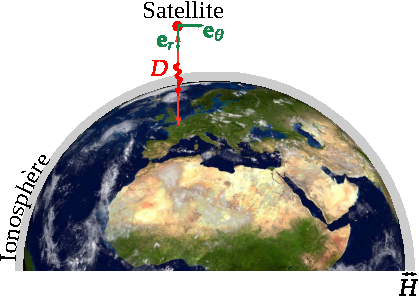
\includegraphics[scale=1.2]{GPS}
	\caption{Lorsqu'un satellite (point rouge) envoie une onde 
		électromagnétique (flèche rouge)
		à un observateur se trouvant à une distance $D$ sur Terre,
		cette dernière doit traverser l'ionosphère (en gris) d'épaisseur
		$H$.}%
	\label{fig:maxwell_GPS}
\end{figure}

L'ionosphère est un plasma, un gaz ionisé, globalement neutre. Il contient :
\begin{itemize}
	\item des électrons de masse $m_e$, de charge $-e$ et de densité particulaire
	  $n_e$ (nombre d'électrons par unité de volume),
	\item d'ions de masse $m_i$, de charge $e$ et de densité particulaire $n_e$.
\end{itemize}
On suppose ici que le plasma est suffisamment dilué pour considérer que ses éléments 
constitutifs sont sans interaction. De plus, les ions ayant une masse beaucoup plus
importantes que les électrons, nous ferons l'hypothèse que ces derniers sont fixes.

On se place dans un repère sphérique $(O, \er, \etheta, \ephi)$ dont l'origine est 
placée au niveau du satellite. On suppose que le satellite génère une onde plane
progressive harmonique de vecteur d'onde complexe $\complex{\vec{k}}$ et de pulsation
temporelle $\omega$. Les champs électrique $\complex{\vece}$ et magnétiques 
$\complex{\vecb}$ en un point $M$ de l'espace de coordonnées $(r, 0, 0)$ 
s'écrivent en notation complexe
\begin{equation*}
	\complex{\vece}(M, t) = \complex{\vece_0} 
	\exp\left[i(\omega t - \complex{k} r
	)\right]
	\quad \mathrm{et} \quad
	\complex{\vecb}(M, t) = \complex{\vecb_0} 
	\exp\left[i(\omega t - \complex{k} r
	)\right],
\end{equation*}
où $\complex{\vece_0}$ et $\complex{\vecb_0}$ sont respectivement 
les amplitudes complexes des champs $\complex{\vece}$ et $\complex{\vecb}$.

\begin{rem}
	On parle ici en réalité d'une onde pseudo progressive 
	car le vecteur d'onde $\vec{k}$ est complexe.
\end{rem}

\subsection{Conductivité complexe}
Dans un premier temps, on cherche à modéliser la réponse de l'ionosphère à cette onde 
électromagnétique. En d'autres termes, on cherche à savoir comment vont réagir les
électrons qui composent cette dernière. Comme nous l'avons fait dans le 
Chapitre~\ref{chap:metaux}, nous allons donc nous intéresser au mouvement d'un électron
du plasma.

\subsubsection{Forces s'exerçant sur un électron du plasma}
On considère un électron du plasma placé en un point $M$.
Cet électron est soumis à
\begin{itemize}
	\item la force de gravitation $\vec{F}_G$ de la Terre,
	\item la force de Lorentz $\vec{F}_L = -e(\vece + \vec{v} \wedge \vecb)$ 
	  résultant du passage de l'onde,
\end{itemize}
où $\vec{v}$ est la vitesse de l'électron. Comme nous l'avons vu précédemment
dans le cours, nous pouvons négliger la force de gravitation devant celle de Lorentz
étant donné la masse d'un électron. On peut de même comparer les deux
termes de la force de Lorentz. Pour cela, nous allons faire l'hypothèse ici que
\begin{equation*}
	||\vecb|| = \dfrac{||\vece||}{c}.
\end{equation*}

\begin{rem}
Cette relation est vrai pour une OPPH électromagnétique dans le vide, mais il n'y a
aucune raison qu'elle le demeure ici. Néanmoins, elle demeure une bonne approximation.
\end{rem}

On obtient alors 
\begin{equation*}
	\dfrac{||\vecv|| \times ||\vecb||}{||\vece||} \approx \dfrac{v}{c}.
\end{equation*}
On peut donc négliger la force magnétique devant la force électrique dès lors
que la vitesse des électrons est non relativiste. Nous poursuivons donc notre 
étude dans un cadre non relativiste. En résumé, l'électron n'est soumis qu'à la
force électrique !

\subsubsection{Principe fondamentale de la dynamique}
On applique maintenant le principe fondamentale de la dynamique à l'électron dans
le référentiel terrestre supposé ici galiléen
\begin{equation*}
	m_e \dn{\vecv}{t} = -e \vece.
\end{equation*}
L'onde électromagnétique étant harmonique, cette équation peut-être mise sous 
une forme complexe
\begin{equation*}
	i \omega m_e \complex{\vecv} = -e \complex{\vece}
	\iff 
	\complex{\vecv} = \dfrac{i e \complex{\vece}}{\omega m_e}.
\end{equation*}
On peut ainsi remonter à une expression reliant le champ électrique 
$\complex{\vece}$ et le vecteur densité de courant $\complex{\vecj}$
\begin{equation*}
	\complex{\vecj} = -e n_e \complex{\vecv} = \dfrac{-i e^2 n_e}{\omega m_e}
	\complex{\vece}.
\end{equation*}
La conductivité $\complex{\gamma}$ étant définie par $\complex{\vecj} =
\complex{\gamma} \complex{\vece}$, on obtient finalement
\begin{equation*}
	\boxed{
	\complex{\gamma} = - \dfrac{i e^2 n_e}{\omega m_e}.
}
\end{equation*}

\subsection{Relation de dispersion du plasma}
Nous sommes maintenant capable d'écrire les équations de Maxwell pour un plasma neutre
(avec une densité volumique de charge $\rho$ nulle) en notation complexe

\begin{description}[labelindent=2em, itemsep=1em]
	\item[Maxwell-Gauss : ]
	 $\complex{\vec{k}} \cdot \complex{\vece} = 0$,
	\item[Maxwell-Thomson : ]
	 $\complex{\vec{k}} \cdot \complex{\vecb} = 0$,
	\item[Maxwell-Faraday : ]
	$\dfrac{\complex{\vec{k}} \wedge \complex{\vece}}{\omega} = \complex{\vecb}$,
	\item[Maxwell-Ampère : ]
		$\complex{\vec{k}} \wedge \complex{\vecb} = i \mu_0 \complex{\vecj}
		+ i \omega \mu_0 \epsilon_0 \complex{\vece}
		= \left(\dfrac{\mu_0 n_e e^2}{m_e \omega} - \dfrac{\omega}{c^2} \right)
		\complex{\vece}$.
\end{description}
On remarque que seule l'équation de Maxwell-Ampère a été modifiée par rapport
aux équations énoncées dans le vide. En utilisant l'équation de Maxwell-Faraday
et l'équation de Maxwell-Ampère, on obtient
\begin{equation*}
	\complex{\vec{k}} \wedge (\complex{\vec{k}} \wedge \complex{\vece})
	= \left(\dfrac{\mu_0 n e^2}{m_e} - \dfrac{\omega^2}{c^2} \right)
	\complex{\vece}.
\end{equation*}
Or, $\complex{\vec{k}} \wedge (\complex{\vec{k}} \wedge \complex{\vece}) = 
(\complex{\vec{k}} \cdot \complex{\vece}) \complex{\vec{k}} - \complex{k}^2
\complex{\vece}$ donc en utilisant Maxwell-Gauss, l'équation précédente devient alors
\begin{equation*}
	\left(\complex{\vec{k}}^2 + \dfrac{\mu_0 n e^2}{m} - \dfrac{w^2}{c^2}\right)
	\complex{\vece} = \vec{0}.
\end{equation*}
On peut alors simplifier le champ électrique car ce dernier n'est pas identiquement
nul. On aboutit alors à la relation de dispersion
\begin{equation}
	\boxed{
	\complex{k}^2 = \dfrac{\omega^2 - \omega_p^2}{c^2}
	\quad \mathrm{avec} \quad \omega_p = \sqrt{\dfrac{n e^2}{\epsilon_0 m}},
}
	\label{eq:plasma}
\end{equation}
où $\omega_p$ est appelée \textbf{pulsation de coupure du plasma}. On obtient 
donc une relation de dispersion qui diffère de celle du vide et qui fait notamment
apparaître une pulsation spécifique $\omega_p$. 

On peut alors se demander ce qu'induit
cette nouvelle relation de dispersion physiquement. On remarque premièrement que si $\omega
< \omega_p$, alors $\complex{k}$ est un imaginaire pur. On peut alors poser 
$\complex{k} = -i k''$ où $k''$ est un réel. Dans notre cas, le champ électrique
devient alors 
\begin{equation*}
	\complex{\vece} = \complex{\vece_0}\exp(-k''z)\exp(i \omega t)
	\Rightarrow \vece = \Re(\complex{\vece}) = \vece_0 \exp(-k''r)\cos(\omega t),
\end{equation*}
où $\Re(\complex{\vece})$ est la partie réelle de $\complex{\vece}$. On obtient
donc une onde dont l'amplitude décroît rapidement avec $r$. Une onde dont la 
pulsation est inférieur à la pulsation de coupure du plasma est incapable de le 
traverser ! On considère pour la suite de l'étude que $\omega > \omega_p$. 
Dans la suite du problème, le vecteur d'onde $\vec{k}$ est donc réel.

\subsection{Paquet d'onde et dispersion}
En réalité, le satellite envoie deux signaux sous la forme de trains d'ondes, c'est-à-dire
des OPPH de taille spatiale finie, de fréquences $f_1$ et $f_2$ pour corriger
l'existence de l'ionosphère. Les fréquences $f_1$ et $f_2$ sont choisies bien supérieures
à la fréquence de coupure du plasma. Pour résoudre
notre problème, il est nécessaire de connaître la vitesse de propagation
des trains d'onde dans l'ionosphère.

%\begin{figure}[t]
%	\centering
%	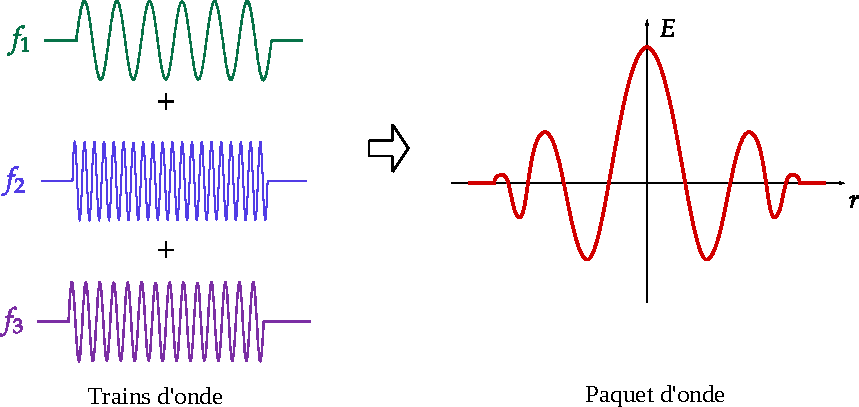
\includegraphics[scale=0.8]{paquet_onde}
%	\caption{Un paquet d'onde (à droite) est formé en additionnant des trains
%	d'ondes (à gauche) de fréquences $f_1$, $f_2$ et $f_3$.}%
%	\label{fig:maxwell_paquet}
%\end{figure}

La vitesse d'un train d'onde est donnée par la \textbf{vitesse de groupe} $v_g$
définie par 
\begin{equation*}
	v_g = \dn{\omega}{k}.
\end{equation*}

\begin{rem}
	Pour une onde, la vitesse de groupe correspond à la vitesse de 
	propagation de l'énergie.
\end{rem}

Dans le vide, $v_g = c$, mais qu'en est-il dans le plasma ? Pour déterminer son 
expression on différencie la relation de dispersion~\ref{eq:plasma}
\begin{equation*}
	k \mathrm{d}k = \dfrac{\omega \mathrm{d}\omega}{c^2}.
\end{equation*}
On obtient alors la vitesse de dispersion
\begin{equation*}
	v_g = \dn{\omega}{k} = \dfrac{k c^2}{\omega} = \dfrac{c \sqrt{\omega^2
	- \omega_p^2}}{\omega} \Rightarrow \boxed{v_g = c 
	\sqrt{1 - \dfrac{\omega_p^2}{\omega^2}}}.
\end{equation*}
Dans le plasma, contrairement au vide, la vitesse de groupe dépend de la pulsation de
l'onde considérée, c'est le phénomène de \textbf{dispersion}.
%Cette dépendance a un impact concret sur le paquet d'onde, il
%va s'étendre spatialement au cours du temps en traversant l'ionosphère, 
%c'est le phénomène de \textbf{dispersion}.

\subsection{Calcul de la distance $D$}
Nous avons pu constater que la propagation d'une onde électromagnétique dans 
un plasma se heurte à deux problèmes majeurs
\begin{enumerate}
	\item la pulsation de l'onde doit être assez élevée pour se propager
	  dans le plasma,
	\item la vitesse de propagation dans le plasma dépend de la pulsation de
	  l'onde.
\end{enumerate}

%Pour simplifier le problème, on imagine que le satellite envoie un paquet d'onde
%composé de trois trains d'ondes de fréquence $f_0$, $f_1$ et $f_2$. On supposera
%ici que ces 3 fréquences sont bien supérieures à la fréquence de coupure
%$f_p$ du plasma. L'onde est donc capable de se propager dans le plasma.
Nous cherchons maintenant à déterminer l'erreur de précision du GPS induite
par la présence de l'ionosphère.

Le train d'onde de fréquence $f_1$ met une durée $\tau$ à parcourir la distance
$D$ qui sépare le satellite du récepteur.
 Ce train d'onde se déplace à la vitesse $c$ dans le vide et à la vitesse 
 $v_g(f_1)$ dans l'ionosphère. $\tau$ est donc donné par 
\begin{equation*}
	\tau = \dfrac{H}{v_g(f_1)} + \dfrac{D - H}{c} = \dfrac{H}{c}
	\left\{\left[1 - \left(\dfrac{f_p}{f_1}\right)^2\right]^{-1/2} - 1 \right\}
	+ \dfrac{D}{c}.
	\approx \boxed{\dfrac{D}{c} \left[1 + \dfrac{H}{2D}\left(\dfrac{f_p}{f_1}\right)^2
	\right]}.
\end{equation*}
La présence de l'ionosphère entraîne donc une augmentation du temps nécessaire
au train d'onde pour arriver au récepteur. Pour corriger l'erreur de précision
du GPS, il suffit de prendre en compte ce retard !
Malheureusement, l'expression de ce dernier fait intervenir l'épaisseur de 
l'ionosphère et sa fréquence de coupure qui sont deux grandeurs difficilement 
mesurables. On cherche donc à s'en débarrasser.

On exprime l'écart $\Delta t$ entre les temps de parcours
du train d'onde de fréquence $f_1$ et de celui de fréquence $f_2$. On a choisi
$f_1$ et $f_2$ telles que $f_1 < f_2$. En s'appuyant sur la formule précédente 
%obtenue pour le train d'onde de fréquence $f_0$, on trouve
\begin{equation*}
	\boxed{\Delta t = \dfrac{H f_p^2}{2c} \dfrac{f_2^2 - f_1^2}{f_2^2f_1^2}.}
\end{equation*}
Cette relation est très intéressante car elle permet d'exprimer l'épaisseur 
de l'ionosphère $H$ en fonction de $\Delta t$ qui est une mesure plus facilement 
accessible au récepteur. On peut alors déterminer avec plus de précision la
distance $D$ qui le sépare du satellite

\begin{equation*}
	D = c \tau - \dfrac{H}{2}\left(\dfrac{f_p}{f_1}\right)^2 = 
	c \tau - \left(\dfrac{f_2 f_1}{f_1}\right)^2 \dfrac{c \Delta t}{ 
	f_2^2 - f_1^2}.
\end{equation*}
Pour prendre en compte l'ionosphère il suffit donc d'appliquer une correction $d$
\begin{equation*}
	\boxed{d = {f_2}^2 \dfrac{c \Delta t}{ 
	f_2^2 - f_1^2}.
 }
\end{equation*}
On réalise l'application numérique avec $f_2 = \unit{1575}{\mega \hertz}$, 
$f_1 = \unit{1228}{\mega \hertz}$
et $\Delta t = \unit{6.7 \times 10^{-7}}{\second}$. On a alors
\begin{equation*}
	d \approx \unit{300}{\meter}.
\end{equation*}
Cette correction doit absolument être prise en compte !
